%%%%%%%%%%%%%%%%%%%%%%%%%%%%%%%%%%%%%%%%%%%%%%%%%%%%%%%%%%%%%%%%%%%%%%
% Problem statement
\begin{statement}[
  problempoints=110,
  timelimit=3 seconds,
  memorylimit=512 MiB,
]{Checker}

``\textit{...fool me once, shame on — shame on you. Fool me — you can't get fooled again.}''
-- W.

In this task, we will observe regular polygons that have each of their $N$ sides
colored in one of three colors and whose vertices are denoted from $1$ to $N$
in a clockwise order. A \textit{triangulaton} of a polygon is a decomposition of
its area into a set of non-overlapping triangles whose sides either lie on the
sides of the polygon or its internal diagonals. Of course, in this task, each of
the diagonals used for polygon triangulation is also colored in one of three
colors.

The triangulation is said to be \textit{patriotic} if each of its $N-2$
triangles has all three sides of different colors. Your task is to determine
whether a given polygon with its diagonals is triangulated and whether that
triangulation is patriotic.

%%%%%%%%%%%%%%%%%%%%%%%%%%%%%%%%%%%%%%%%%%%%%%%%%%%%%%%%%%%%%%%%%%%%%%
% Input
\subsection*{Ulazni podaci}
The frist line contains the number of subtask this particular test case belongs
to (see the table in the scoring section). If your solution doesn't care about
that, simply read the number and feel free to ignore it.

The second line contains an integer $N$ from the task description.

The third line contains an integer consisting of $N$ digits which represent
the colors of polygon sides. More precisely, the first digit represents
the color of side $(1,2)$, the second digit represents the color of side $(2,3)$,
and so on until the $N$-th digit which represents the color of side $(N,1)$. The
colors will always be denoted with digits $1$, $2$ and $3$.

Each of the next $N-3$ lines contain a description of one diagonal in
the form $X$ $Y$ $C$, where $X$ and $Y$ are polygon vertices and
$C$ is the color of the diagonal $(1 \le X, Y \le N, 1 \le C \le 3)$. Each
line describes a valid diagonal, i.e., vertices $X$ and $Y$ will neither
be equal nor neighbouring.

%%%%%%%%%%%%%%%%%%%%%%%%%%%%%%%%%%%%%%%%%%%%%%%%%%%%%%%%%%%%%%%%%%%%%%
% Output
\subsection*{Output}
If the input polygon is not correctly triangulated, you should output
\texttt{"neispravna triangulacija"} (invalid triangulation in Croatian).

If the input polygon is correctly triangulated but the triangulation is
not patriotic, you should output \texttt{"neispravno bojenje"} (invalid
coloring in Croatian).

If the input polygon is correctly triangulated and that triangulation is
patriotic, you should output \texttt{"tocno"} (correct in Croatian).

%%%%%%%%%%%%%%%%%%%%%%%%%%%%%%%%%%%%%%%%%%%%%%%%%%%%%%%%%%%%%%%%%%%%%%
% Scoring
\subsection*{Scoring}
{\renewcommand{\arraystretch}{1.4}
  \setlength{\tabcolsep}{6pt}
  \begin{tabular}{ccl}
 Subtask & Score & Constraints \\ \midrule
  1 & 12 & $4 \le N \le 300$ \\
  2 & 17 & $4 \le N \le 2000$ \\
  3 & 23 & $4 \le N \le 2\cdot10^5$, the output is either \texttt{neispravna triangulacija} or \texttt{tocno} \\
  4 & 23 & $4 \le N \le 2\cdot10^5$, the output is either \texttt{neispravno bojenje} or \texttt{tocno} \\
  5 & 35 & $4 \le N \le 2\cdot10^5$
\end{tabular}}

Unlike the task \textit{Trobojnica} from round 1, if your program correctly
outputs the first line in each test case of a certain subtask, you will score
$100\%$ of the points allocated for that subtask.

%%%%%%%%%%%%%%%%%%%%%%%%%%%%%%%%%%%%%%%%%%%%%%%%%%%%%%%%%%%%%%%%%%%%%%
% Examples
\subsection*{Examples}
\begin{tabularx}{\textwidth}{X'X'X}
\sampleinputs{test/checker.dummy.in.1}{test/checker.dummy.out.1} &
\sampleinputs{test/checker.dummy.in.2}{test/checker.dummy.out.2} &
\sampleinputs{test/checker.dummy.in.3}{test/checker.dummy.out.3}
\end{tabularx}

\textbf{Clarifications of examples:}

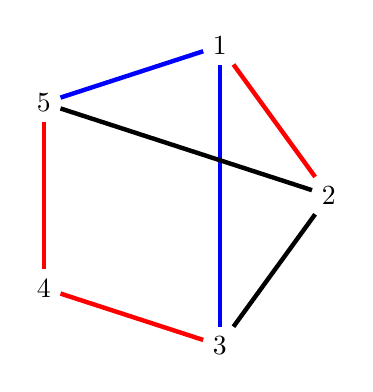
\begin{tikzpicture}
    \def\r{2}

    \node(1) at (1*360/5:\r) {1};
    \node(2) at (0*360/5:\r) {2};
    \node(3) at (4*360/5:\r) {3};
    \node(4) at (3*360/5:\r) {4};
    \node(5) at (2*360/5:\r) {5};

    \draw [ultra thick, red]   (1) -- (2);
    \draw [ultra thick, black] (2) -- (3);
    \draw [ultra thick, red]   (3) -- (4);
    \draw [ultra thick, red]   (4) -- (5);
    \draw [ultra thick, blue]  (5) -- (1);

    \draw [ultra thick, blue]  (1) -- (3);
    \draw [ultra thick, black] (2) -- (5);
\end{tikzpicture}
\hspace{30pt}
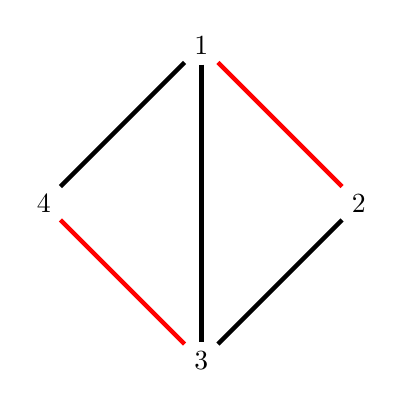
\begin{tikzpicture}
    \def\r{2}

    \node(1) at (1*360/4:\r) {1};
    \node(2) at (0*360/4:\r) {2};
    \node(3) at (3*360/4:\r) {3};
    \node(4) at (2*360/4:\r) {4};

    \draw [ultra thick, red]   (1) -- (2);
    \draw [ultra thick, black] (2) -- (3);
    \draw [ultra thick, red]   (3) -- (4);
    \draw [ultra thick, black] (4) -- (1);

    \draw [ultra thick, black] (1) -- (3);
\end{tikzpicture}
\hspace{30pt}
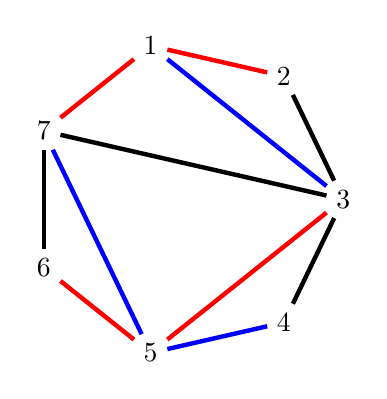
\begin{tikzpicture}
    \def\r{2}

    \node(1) at (2*360/7:\r) {1};
    \node(2) at (1*360/7:\r) {2};
    \node(3) at (0*360/7:\r) {3};
    \node(4) at (6*360/7:\r) {4};
    \node(5) at (5*360/7:\r) {5};
    \node(6) at (4*360/7:\r) {6};
    \node(7) at (3*360/7:\r) {7};

    \draw [ultra thick, red]   (1) -- (2);
    \draw [ultra thick, black] (2) -- (3);
    \draw [ultra thick, black] (3) -- (4);
    \draw [ultra thick, blue]  (4) -- (5);
    \draw [ultra thick, red]   (5) -- (6);
    \draw [ultra thick, black] (6) -- (7);
    \draw [ultra thick, red]   (7) -- (1);

    \draw [ultra thick, blue]  (1) -- (3);
    \draw [ultra thick, red]   (3) -- (5);
    \draw [ultra thick, blue]  (5) -- (7);
    \draw [ultra thick, black] (7) -- (3);
\end{tikzpicture}

%%%%%%%%%%%%%%%%%%%%%%%%%%%%%%%%%%%%%%%%%%%%%%%%%%%%%%%%%%%%%%%%%%%%%%
% We're done
\end{statement}

%%% Local Variables:
%%% mode: latex
%%% mode: flyspell
%%% ispell-local-dictionary: "croatian"
%%% TeX-master: "../hio.tex"
%%% End:
